\chapter{Metodología y método de trabajo}
\label{cap:metodologia}

En este capítulo se explica la metodología de desarrollo que se ha seguido, describiendo desde la captura de requisitos hasta el producto final. Al final del capítulo se añade un apartado con el análisis de costes.

\section{Metodología de desarrollo}

Para organizar el proyecto y permitir un desarrollo eficaz e incremental se ha seguido una metodología de desarrollo en espiral: el \gls{pud}\cite{pud} y \cite{apuntes}.

\subsection{Características principales}
El \gls{pud} es una metodología de desarrollo que transforma los requisitos de usuario en un sistema software. Es muy genérica, y por eso se ha decidido adaptar a este proyecto.
Las características básicas del \gls{pud} son las siguientes:
\begin{itemize}
	\item \textbf{Dirigido por casos de uso:} en este proyecto, los usuarios, como se ha mencionado anteriormente, son los maestros y profesores de \gls{eso}. Los casos de uso que se han contemplado para el proyecto son las acciones que se han especificado en \ref{cap:Introduccion}. Se hablará de la metodología seguida para la captura de requisitos más adelante.
	\item \textbf{Centrado en la arquitectura:} una de las primeras fases del proyecto es realizar el esquema de la base de datos y la comprensión de la futura arquitectura del programa. Esto determinará el orden en el que se desarrollarán los casos de uso.
	\item \textbf{Iterativo e incremental:} se ha trabajado mediante iteraciones, en la que cada una o bien añadía una nueva funcionalidad, mejoraba una de las ya existentes, o realizaba pruebas de cohesión entre los módulos recién añadidos y los que ya estaban desarrollados. También cabe notar que el método de iteraciones ha sido el de terminar por completo una parte, hasta las pruebas, antes de comenzar con otra nueva. En cada iteración en la que se añade una nueva funcionalidad:
	\begin{enumerate}
		\item Se elige una de las que todavía no se han desarrollado.
		\item Dentro de la funcionalidad, se identifican y especifican los casos de uso que le corresponden.
		\item Se refinan los diseños que se hicieron al principio del proyecto para estos casos de uso.
		\item Se implementan y se prueban dentro del módulo de manera que satisfaga de manera vaga los requisitos.
	\end{enumerate}
	
	En cada iteración en la que se mejora una funcionalidad existente:
	\begin{enumerate}
		\item Se elige una de las funcionalidades a probar.
		\item Se prueba exhaustivamente dentro de su módulo para identificar los errores actuales y posibles futuros, y se arreglan los fallos.
	\end{enumerate}
	
	En cada iteración en la que se prueba la cohesión entre los módulos:
	\begin{enumerate}
		\item Se elige uno de los módulos, preferentemente el último que se ha desarrollado.
		\item Se prueba con el resto de los módulos con los que mantiene cualquier tipo de comunicación, se identifican los errores y se arreglan los fallos.
	\end{enumerate}
	
	\item \textbf{Enfocado en los riesgos:} primero se han desarrollado los casos de uso más grandes que, después del primer diseño, se consideró que tendrían más impacto en el programa. Seguidamente, se fue trabajando desarrollando los distintos módulos, uno por cada funcionalidad y una iteración por funcionalidad.
	
\end{itemize}

\subsection{Etapas del proyecto}

Esta metodología consiste en la división del proyecto en cuatro etapas:
\begin{itemize}
    \item \textbf{Inicio:} para comenzar, se han recogido todos los requisitos y se ha estimado el alcance del proyecto. En esta etapa también se hizo la investigación de las aplicaciones ya existentes, descritas en el capítulo \ref{cap:aplicacionesexistentes} y el análisis de costes, desglosado en la sección \ref{analisiscostes}.
    \item \textbf{Elaboración:} se hicieron prototipos de las interfaces, se diseñó el software mediante diagramas y se estimaron las iteraciones a seguir.
    \item \textbf{Construcción:} se escribió el software según el resultado de la fase de elaboración, siguiendo las iteraciones previamente calculadas. 
    \item \textbf{Transición:} para finalizar se probó el producto final y se dio fin al desarrollo.
\end{itemize}

\subsection{Obtención de requisitos}
\label{sub:obtencionrequisitos}

Para la obtención y clasificación de los requisitos, se optará por varias metodologías:
\begin{itemize}
	\item \textbf{Observación activa:} se estudiará el entorno de trabajo del usuario final. Para ello, se realizó una sesión en la que se monitorizó a un usuario usando una de las herramientas descritas en el capítulo Aplicaciones existentes, preguntándole sus opiniones sobre algunas de las características que estaba utilizando.
	\item \textbf{Entrevistas:} entrevistas con el usuario en las que irá evaluando el producto final de cada sprint y añadiendo o modificando características.
\end{itemize}

Además, se ha aplicado la regla MoSCoW para priorizar el desarrollo de los requisitos funcionales. Esta regla divide los requisitos en cuatro categorías:
\begin{enumerate}
	\item \textbf{Must have (M):} requisitos que la aplicación debe tener y son prioritarios a cualquier otro de menor rango.	
	\item \textbf{Should have (S):} estos requisitos, de menor rango que los Must have, siguen siendo requisitos importantes para el desarrollo de la aplicación.	
	\item \textbf{Could have (C):} requisitos de más baja prioridad, que pueden posponerse si hay otros de mayor rango por encima de ellos.	
	\item \textbf{Won't have (W):} requisitos completamente opcionales que la aplicación podría llegar a tener de manera que mejorasen las funcionalidades.
	
\end{enumerate}

\section{Sprints}

A continuación se detallan los sprints que se realizaron en el proyecto. Cabe notar que este documento se escribió al mismo tiempo que se iban desarrollando.

El proyecto, que ha tenido una duración aproximada de 350 horas, se ha desarrollado desde el 2 de octubre de 2020 hasta el 1 de julio de 2021.

\subsection{Primer sprint - 2oct/1nov}

En el primer sprint (2 octubre 2020 - 1 noviembre 2020), al que se dedicaron 30 horas, se refinaron los diseños de la aplicación con la herramienta Balsamiq Wireframes [Sección \ref{sec:prototipos}]. Estos diseños se han modificado varias veces a lo largo de este primer sprint. Además, se realizó el primer diseño de la base de datos [Figura \ref{Fig:db_definition1}].

\begin{figure}[h]
\centering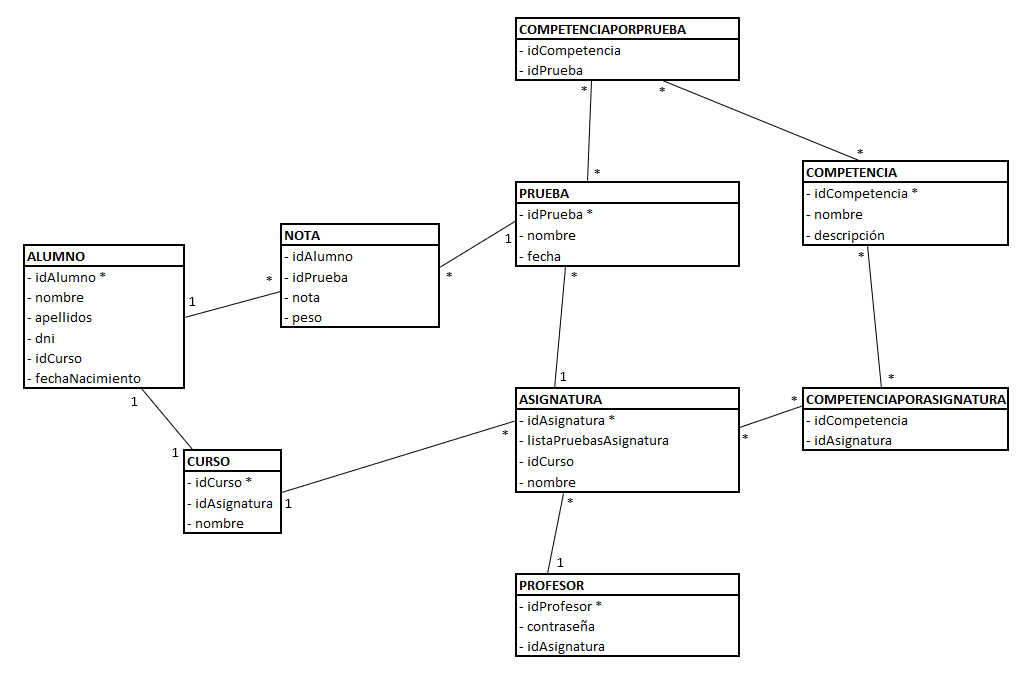
\includegraphics[width=1\linewidth]{figs/DB_Definition_1.png}
\caption{Primera definición de la base de datos.}
\label{Fig:db_definition1}
\end{figure}

\subsection{Segundo sprint - 2nov/1dic}

En el segundo sprint (2 noviembre 2020 - 1 diciembre 2020), al que se dedicaron 20 horas, se comenzó a escribir la memoria del proyecto, empezando por describir las aplicaciones existentes investigadas.

Se siguió trabajando en la base de datos, implementándola mediante MySQL [Sección \ref{sub:mysql}], y comenzó a poblarse de datos de prueba para comenzar el desarrollo.


\subsection{Tercer sprint - 2dic/1ene}

En el tercer sprint (2 diciembre 2020 - 1 febrero 2021), al que se dedicaron 50 horas, se comenzó la implementación de la aplicación por la ventana principal, debido a que al estar unida a todas las funcionalidades del sistema, se consideró la más importante.

Al final de este sprint se decidió cambiar de \gls{ide} de IntelliJ a NetBeans, que es el que se terminó usando para el resto del proyecto, debido a la gran dificultad para trabajar con interfaces en Java con IntelliJ.

\subsection{Cuarto sprint - 2feb/1may}

En el cuarto sprint (2 febrero 2021 - 1 mayo 2021), al que se dedicaron 175 horas, se continuó con el desarrollo de la ventana principal. Cabe notar que en este sprint se decidió dejar las mejoras del diseño de la ventana para sprints posteriores y comenzar con el desarrollo de las funcionalidades principales:
\begin{itemize}
	\item \textbf{Crear una nueva tarea o prueba}, accesible mediante un botón en la ventana principal.
	\item \textbf{Calificar tareas o pruebas}, accesible de la misma manera, con un botón en la ventana principal.
	\item \textbf{Ver informe del alumno}, ventana que se puede acceder al hacer clic en el nombre de un alumno en la tabla.
	\item \textbf{Ver informe del trimestre}, ventana que se puede acceder al hacer clic en el título de un trimestre en la tabla.
\end{itemize}


Al final de este sprint, se comprobó que las funcionalidades desarrolladas se integraban y funcionaban correctamente entre ellas y la ventana principal.

\subsection{Sexto sprint - 2may/1jul}

En el sexto sprint (2 mayo 2021 - 1 julio 2021), al que se dedicaron 75 horas, se realizaron pequeños desarrollos en la aplicación, tanto para añadir nuevas funcionalidades de los apartados de requisitos Could have y Won't have, como para pulir las ya existentes.

En este sprint se desarrollaron las siguientes funcionalidades y se hicieron varios arreglos:
\begin{itemize}
	\item \textbf{Modificación de los datos del docente}, accesibles mediante un botón en la ventana principal.
	\item \textbf{Manual de ayuda}, una pequeña ventana con texto explicando al usuario cada funcionalidad de la aplicación. Es accesible mediante cualquier ventana.
	\item \textbf{Añadir alumnos}, funcionalidad posible mediante un formulario, para un solo alumno, o subiendo un Excel, para varios. Accesible mediante la ventana principal.	
\end{itemize}

Durante este periodo de tiempo también se diseñaron las imágenes e iconos usados en la aplicación.

Por último, en este sprint se decidió implementar las estadísticas para las notas en la ventana principal y la ventana de calificar tareas.

	
\section{Prototipos de interfaces}
\label{sec:prototipos}
En las figuras \ref{Fig:mockup_mainwindow}, \ref{Fig:mockup_nuevatarea} y \ref{Fig:mockup_informealumno} se muestran algunos de los prototipos que se hicieron en la fase de elaboración para las interfaces del programa mediante la herramienta Balsamiq Wireframes\ref{sub:balsamiq}.

\begin{figure}[h]
\centering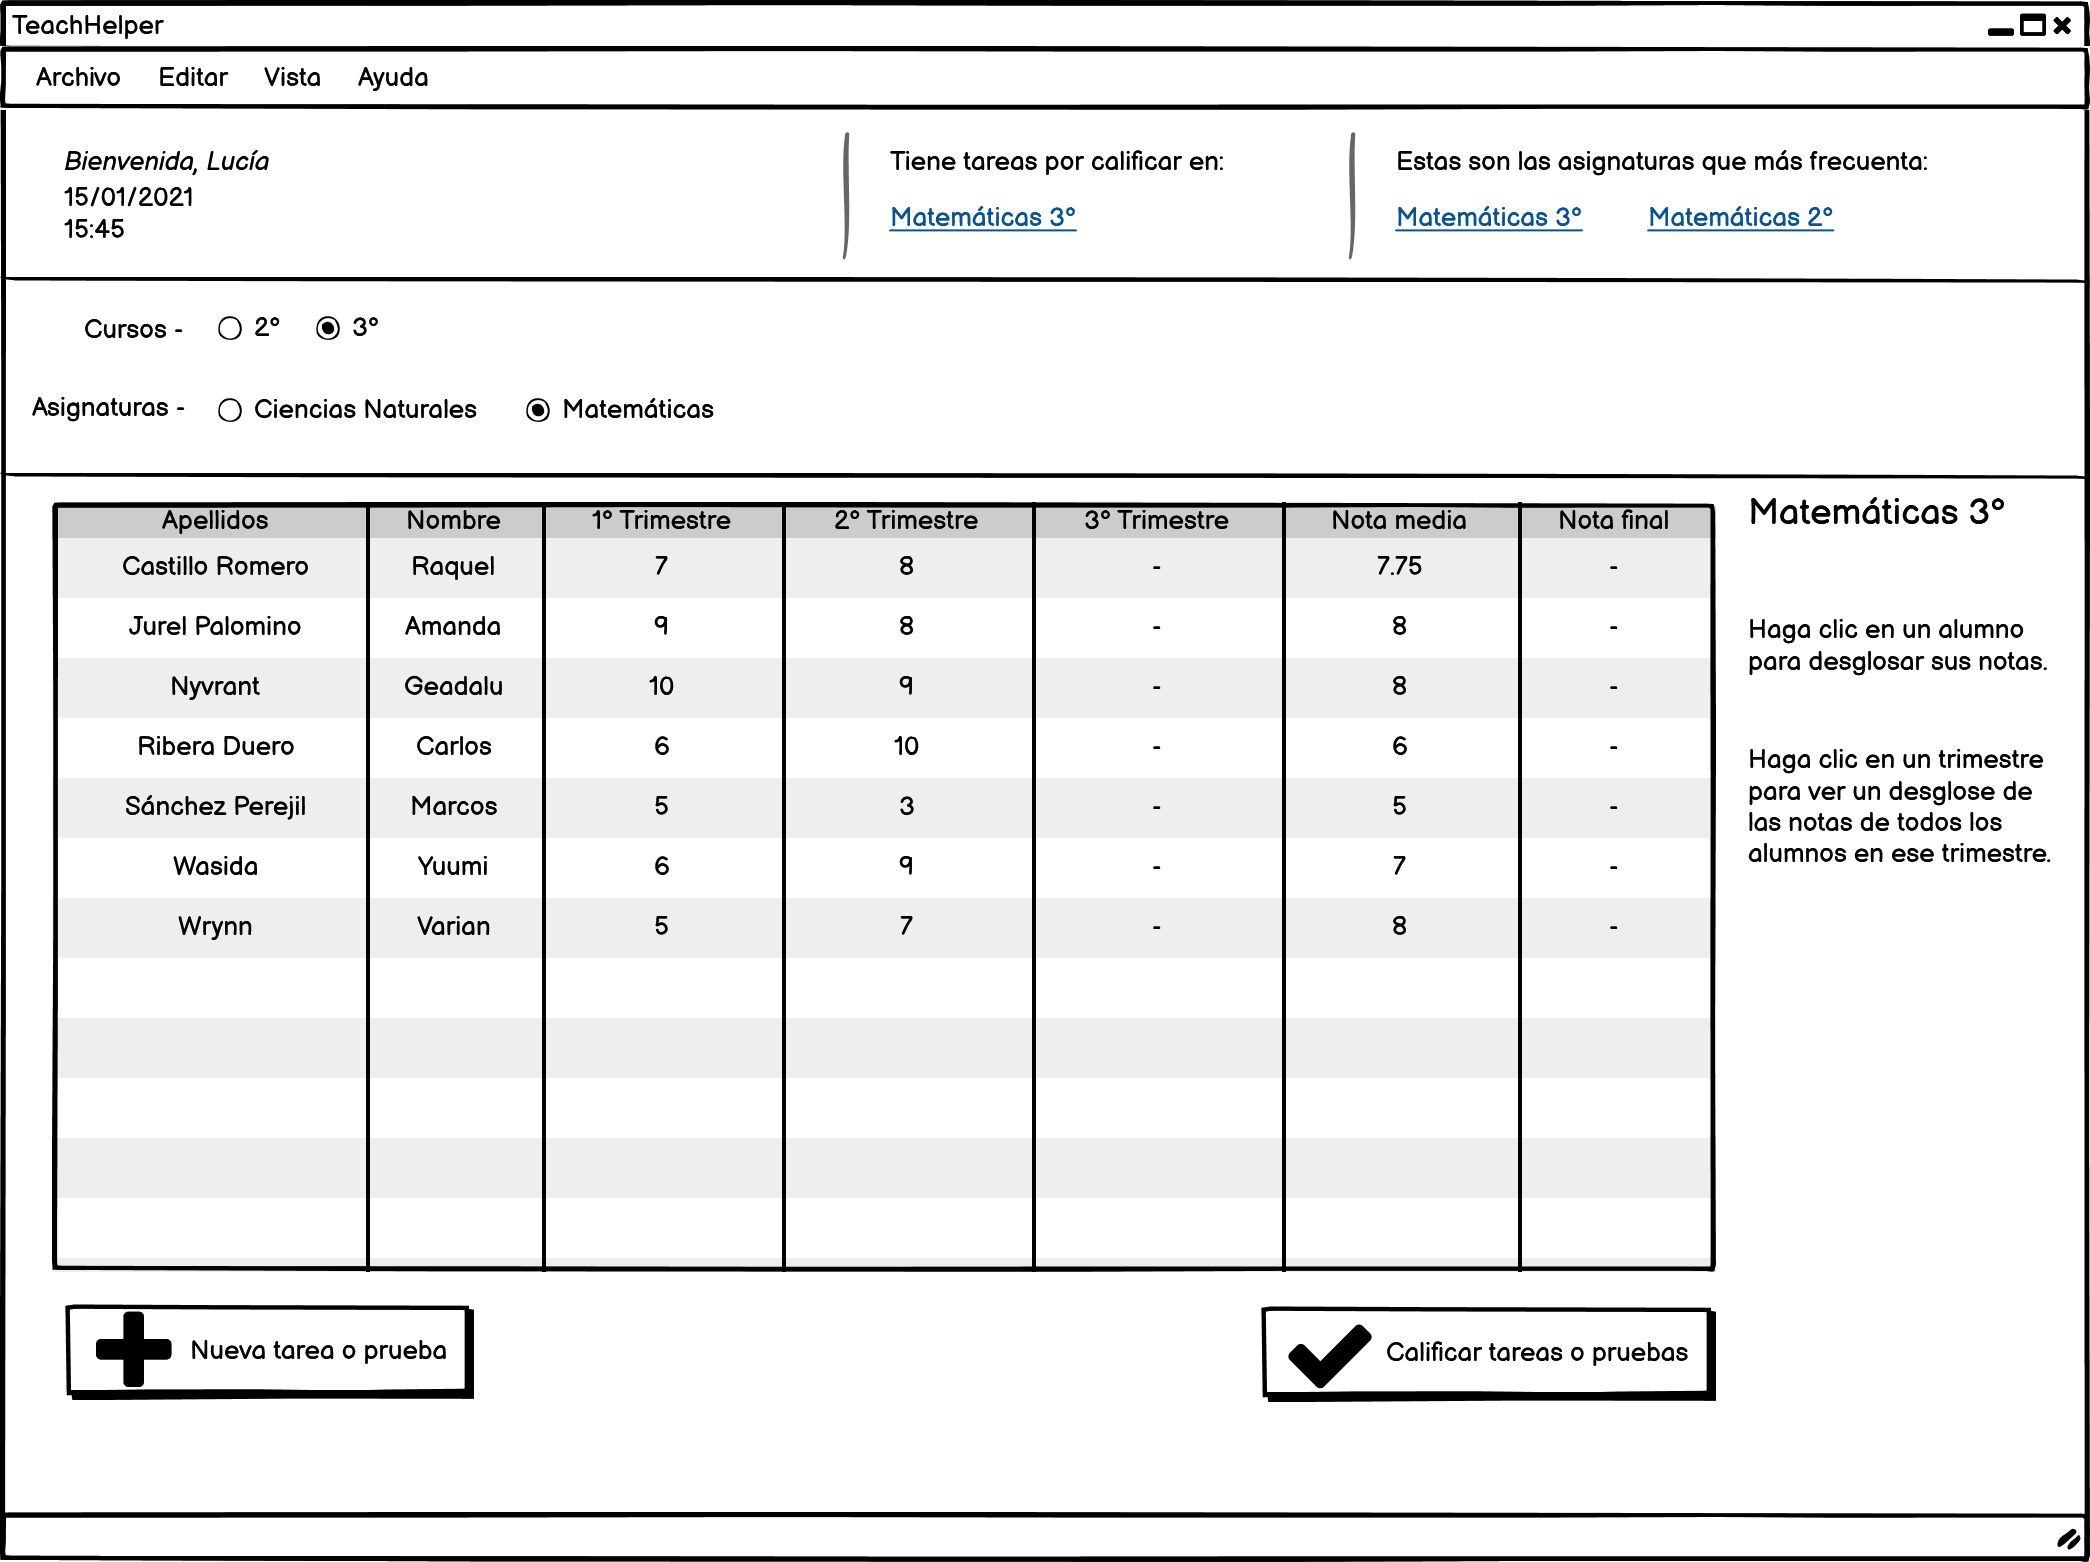
\includegraphics[width=1\linewidth]{figs/mockup_mainwindow.png}
\caption{Prototipo de la ventana principal.}
\label{Fig:mockup_mainwindow}
\end{figure}

\begin{figure}[h]
\centering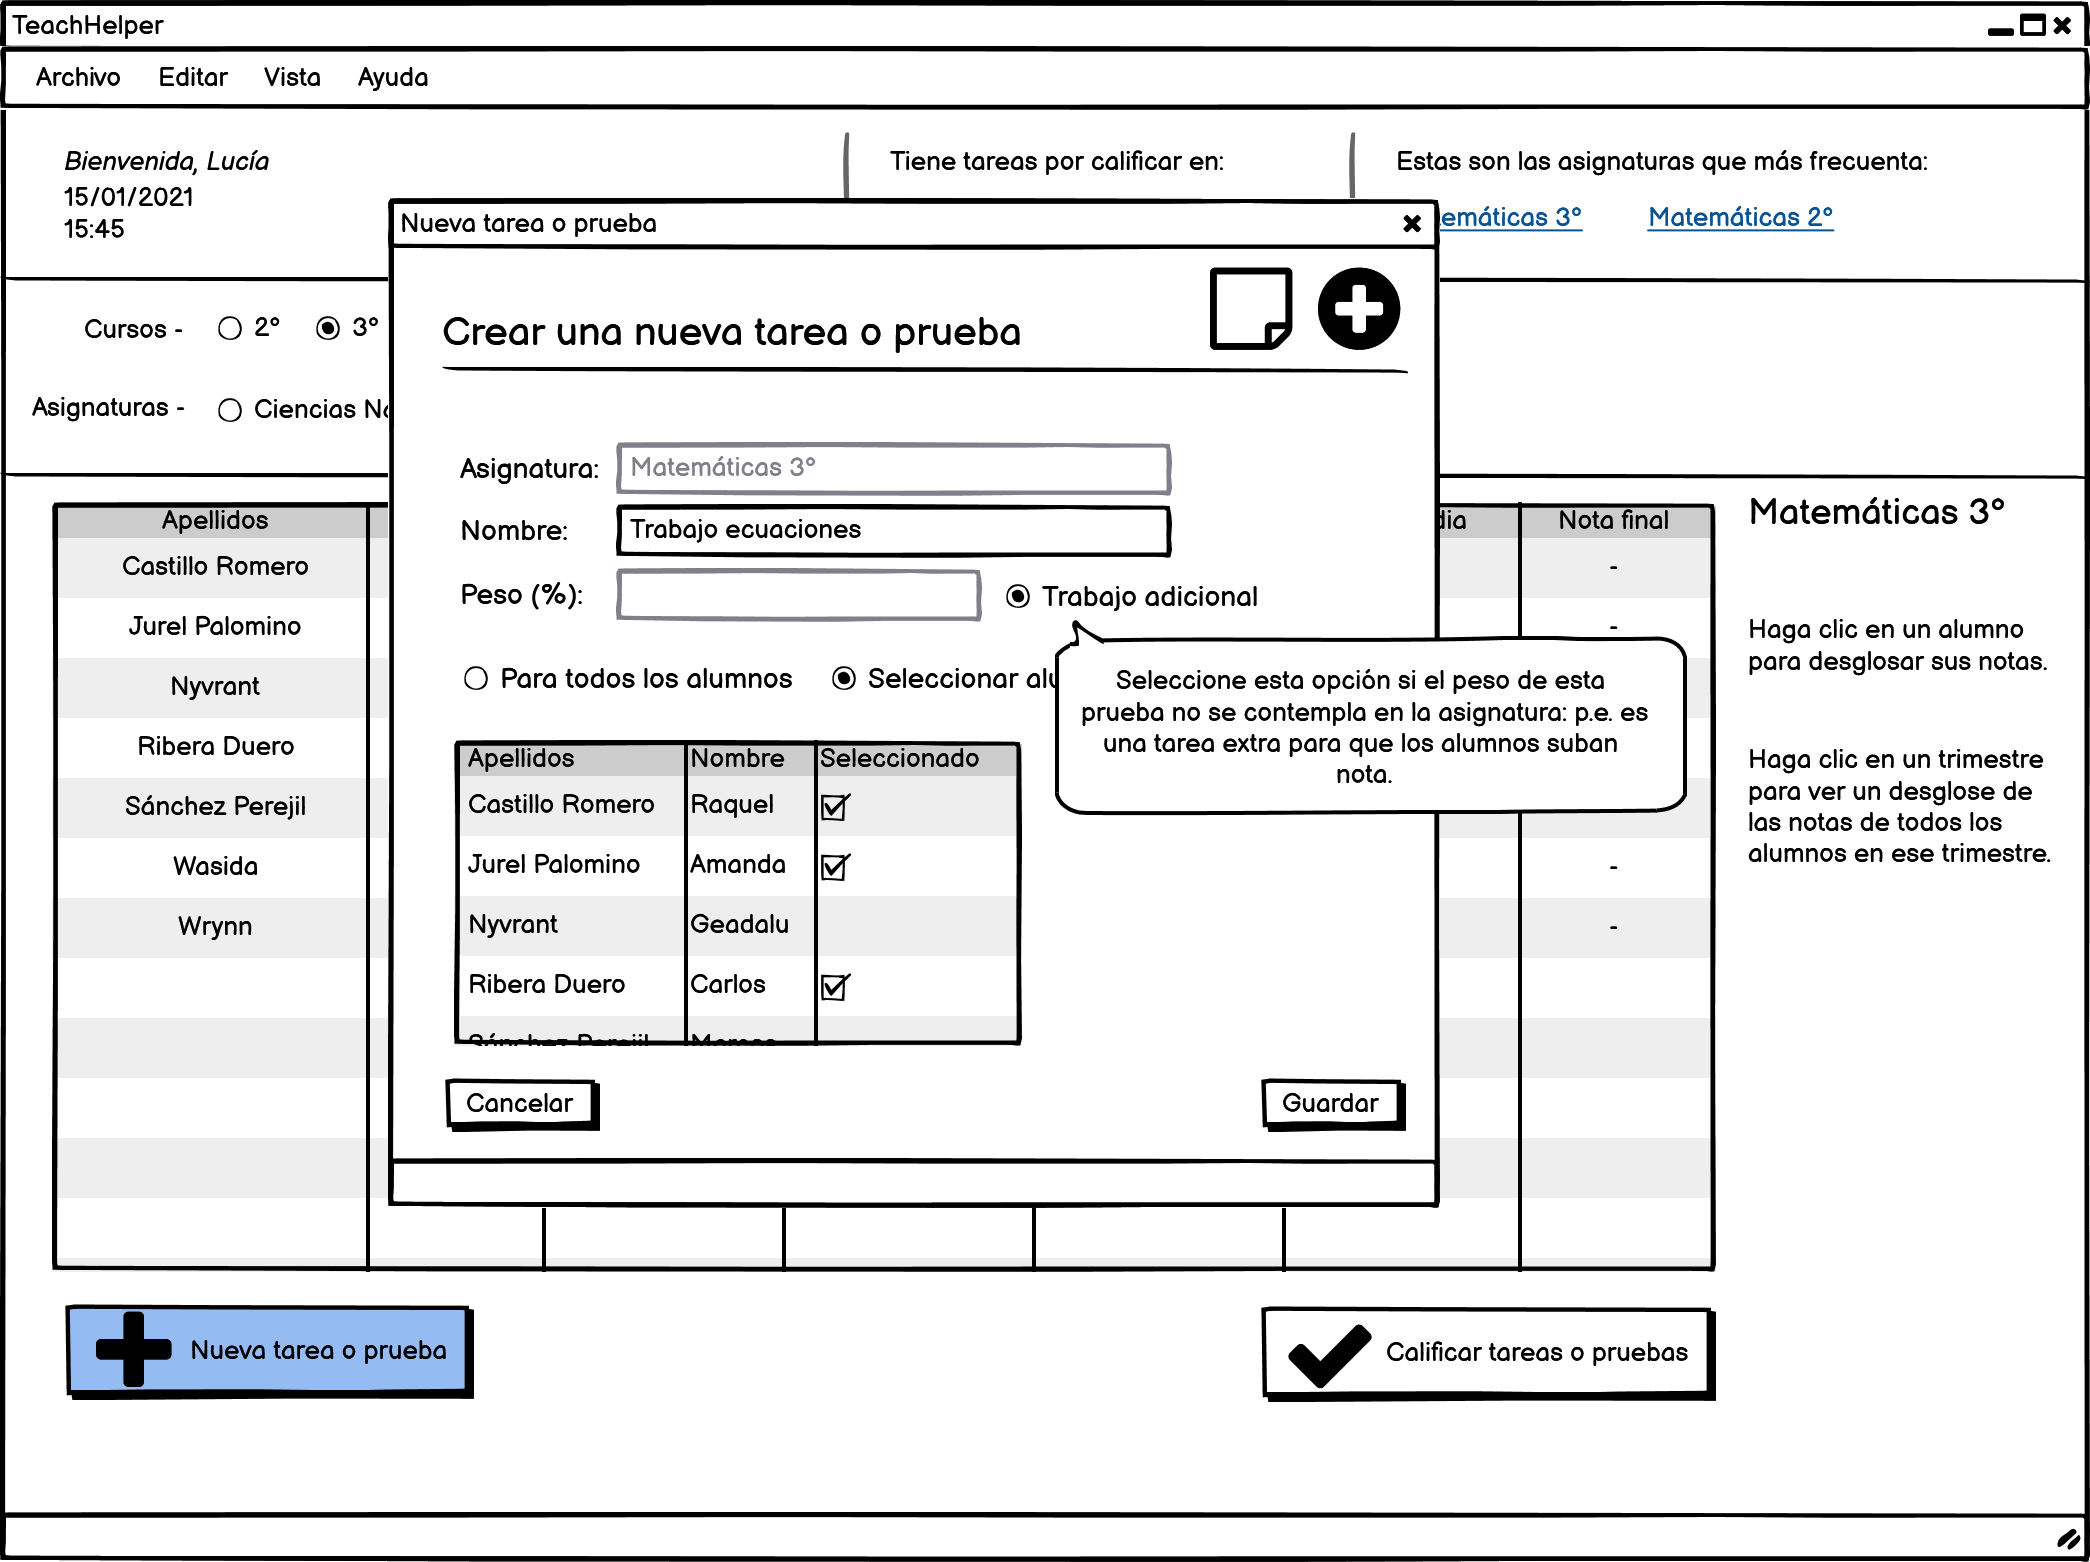
\includegraphics[width=1\linewidth]{figs/mockup_nuevatarea.png}
\caption{Prototipo de la creación de nuevas tareas o pruebas.}
\label{Fig:mockup_nuevatarea}
\end{figure}

\begin{figure}[h]
\centering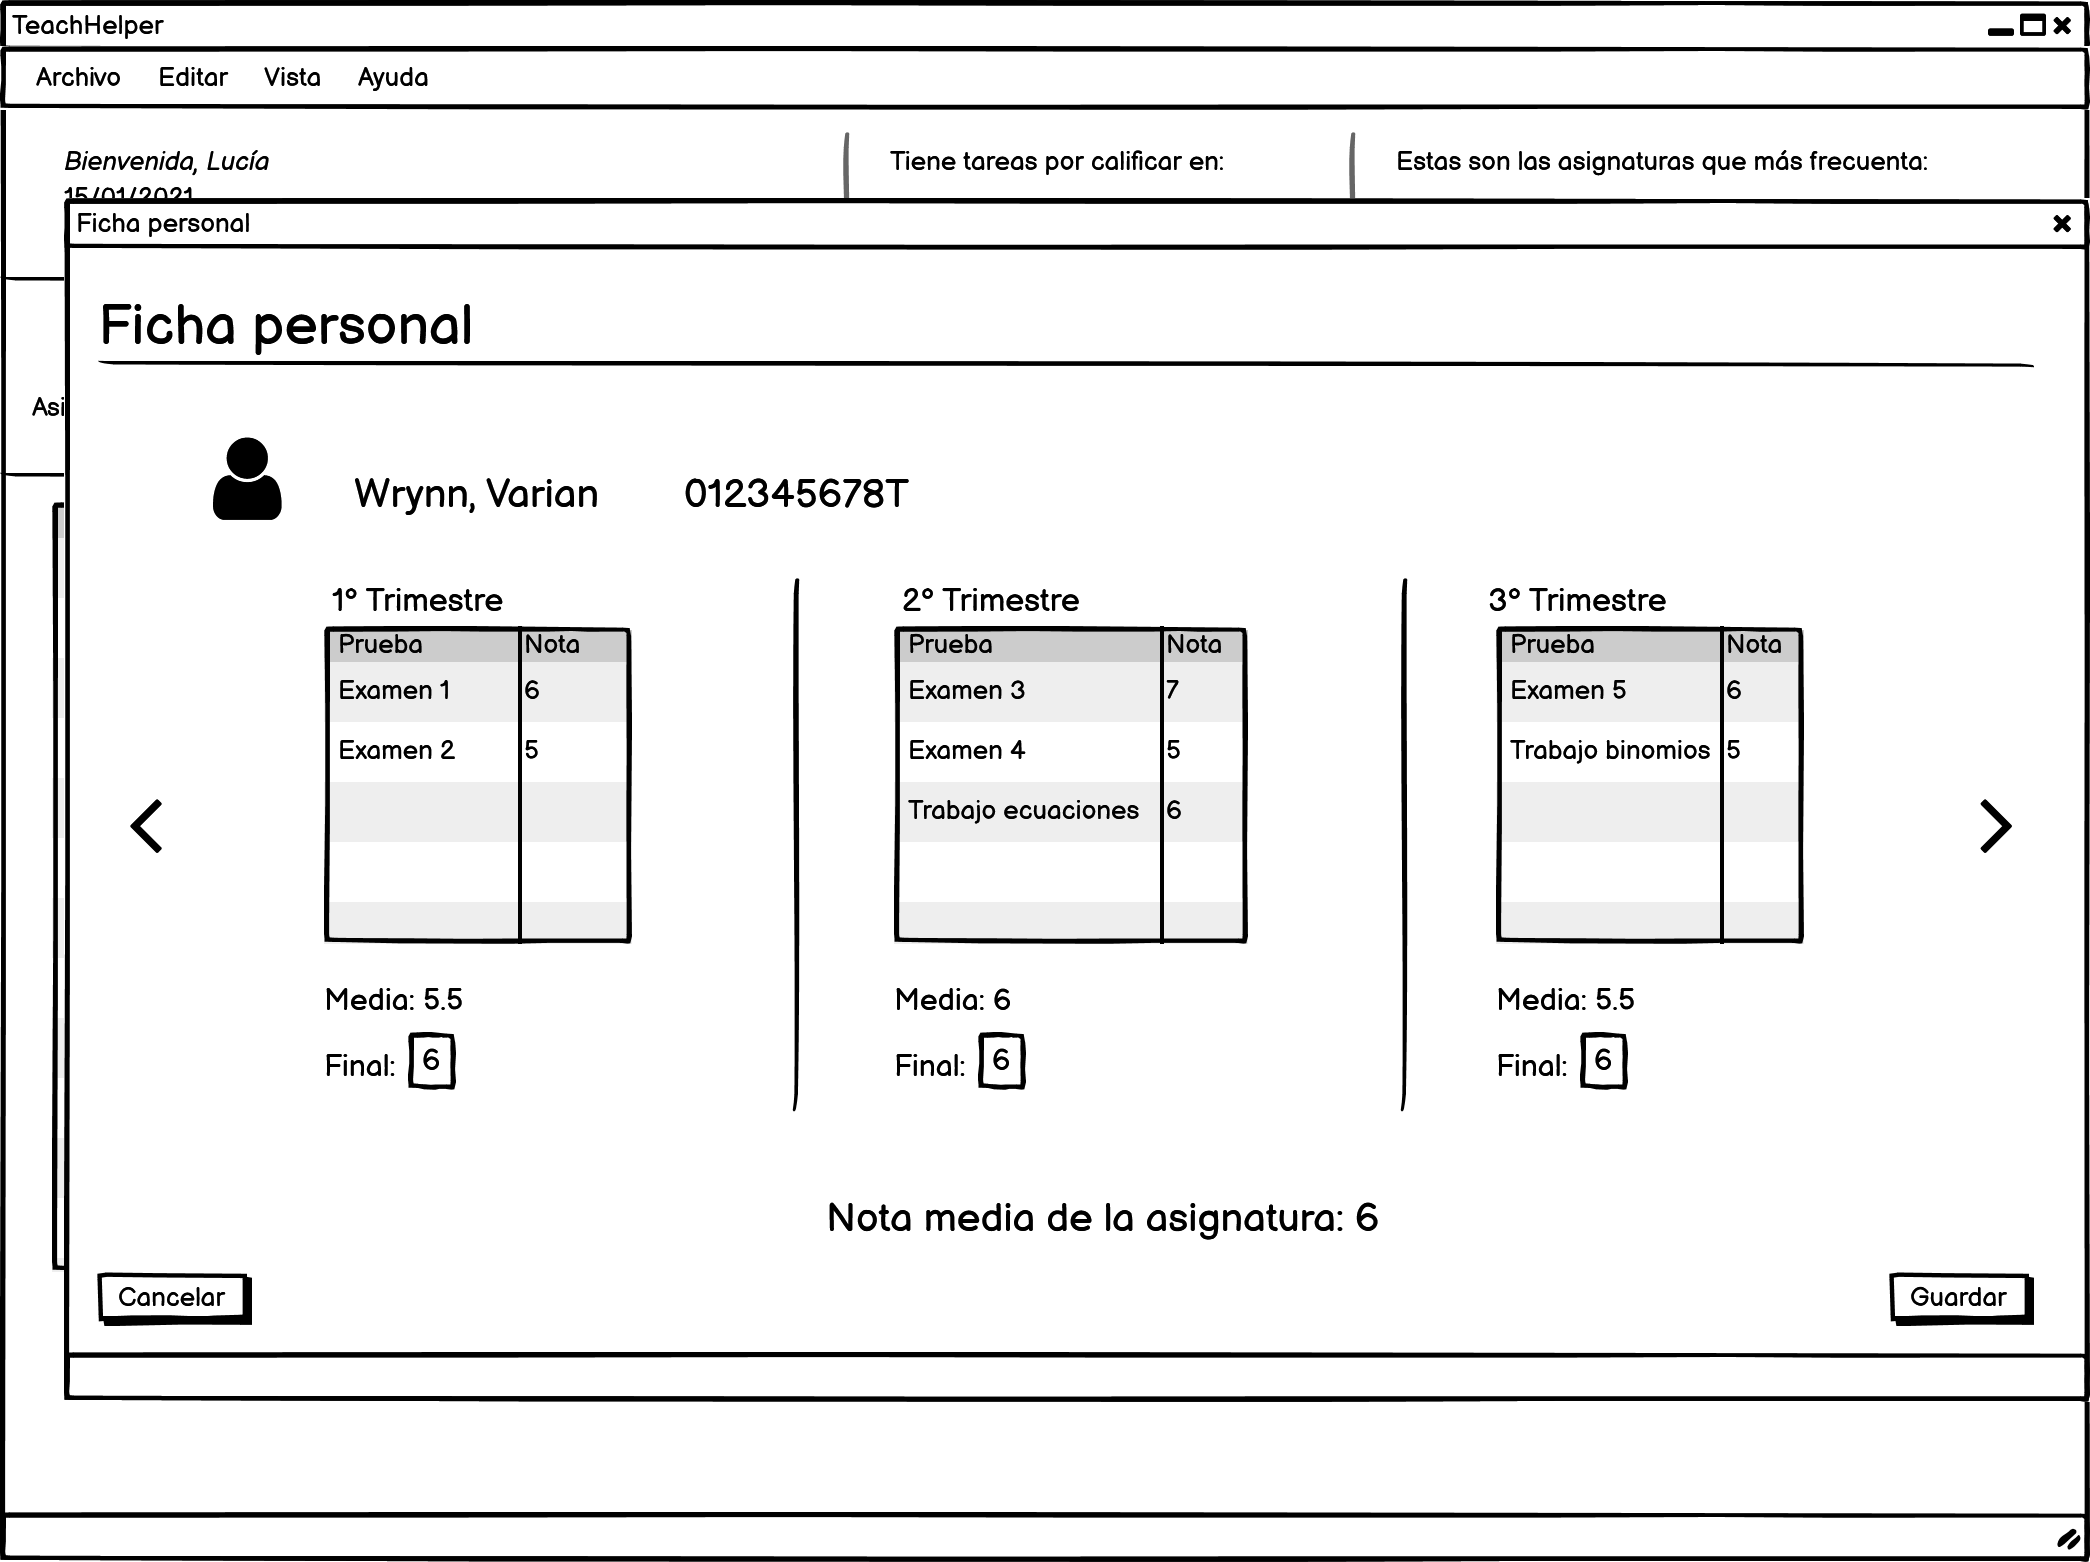
\includegraphics[width=1\linewidth]{figs/mockup_informealumno.png}
\caption{Prototipo del informe del alumnado.}
\label{Fig:mockup_informealumno}
\end{figure}


\section{Marco tecnológico de trabajo}

En esta sección se detallan las tecnologías usadas para el desarrollo de la aplicación.

\subsection{Java}
En la fase de Inicio del proyecto se estudió qué lenguaje de programación utilizar para su desarrollo. Al principio se propuso C\#, pero debido a las restricciones de horario de la desarrolladora y su previo conocimiento de Java (fuente: \cite{java}), se optó finalmente por el segundo.

Otra de las razones por las que se decantó por Java para realizar el proyecto fue la facilidad con la que se crean y modifican las interfaces gráficas con este lenguaje, concretamente si se usa un \gls{ide}.

A continuación se muestra una lista describiendo brevemente las librerías externas que se han usado en el desarrollo de este proyecto.
\begin{itemize}
	\item \textbf{Apache Poi}: permite crear y modificar archivos Microsoft Excel \cite{apachepoi}.
	\item \textbf{JFreeChart}: crea diagramas y gráficos y permite personalizarlos de varias maneras \cite{jfreechart}.
\end{itemize}

\subsection{Git y GitHub}
Se ha usado una herramienta de control de versiones llamada Git (fuente: \cite{git}). Esta herramienta permite subir el código a un repositorio, elegir los cambios que se quieren subir y deshacer los que se han hecho en caso de error. Ha sido de gran ayuda para gestionar el código y las iteraciones correctamente.

Este es el enlace al proyecto en GitHub: https://github.com/Geadalu/MisNotasCode.

Otra razón por la que se ha optado por Git es porque, desde su página web \url{www.github.com}, permite un control de "Issues" o problemas (ver figura \ref{Fig:issues_github}). Esto se ha usado de manera constante para tener mejor control de los errores que iban saliendo en el programa tras las iteraciones de desarrollo.

\begin{figure}[h]
\centering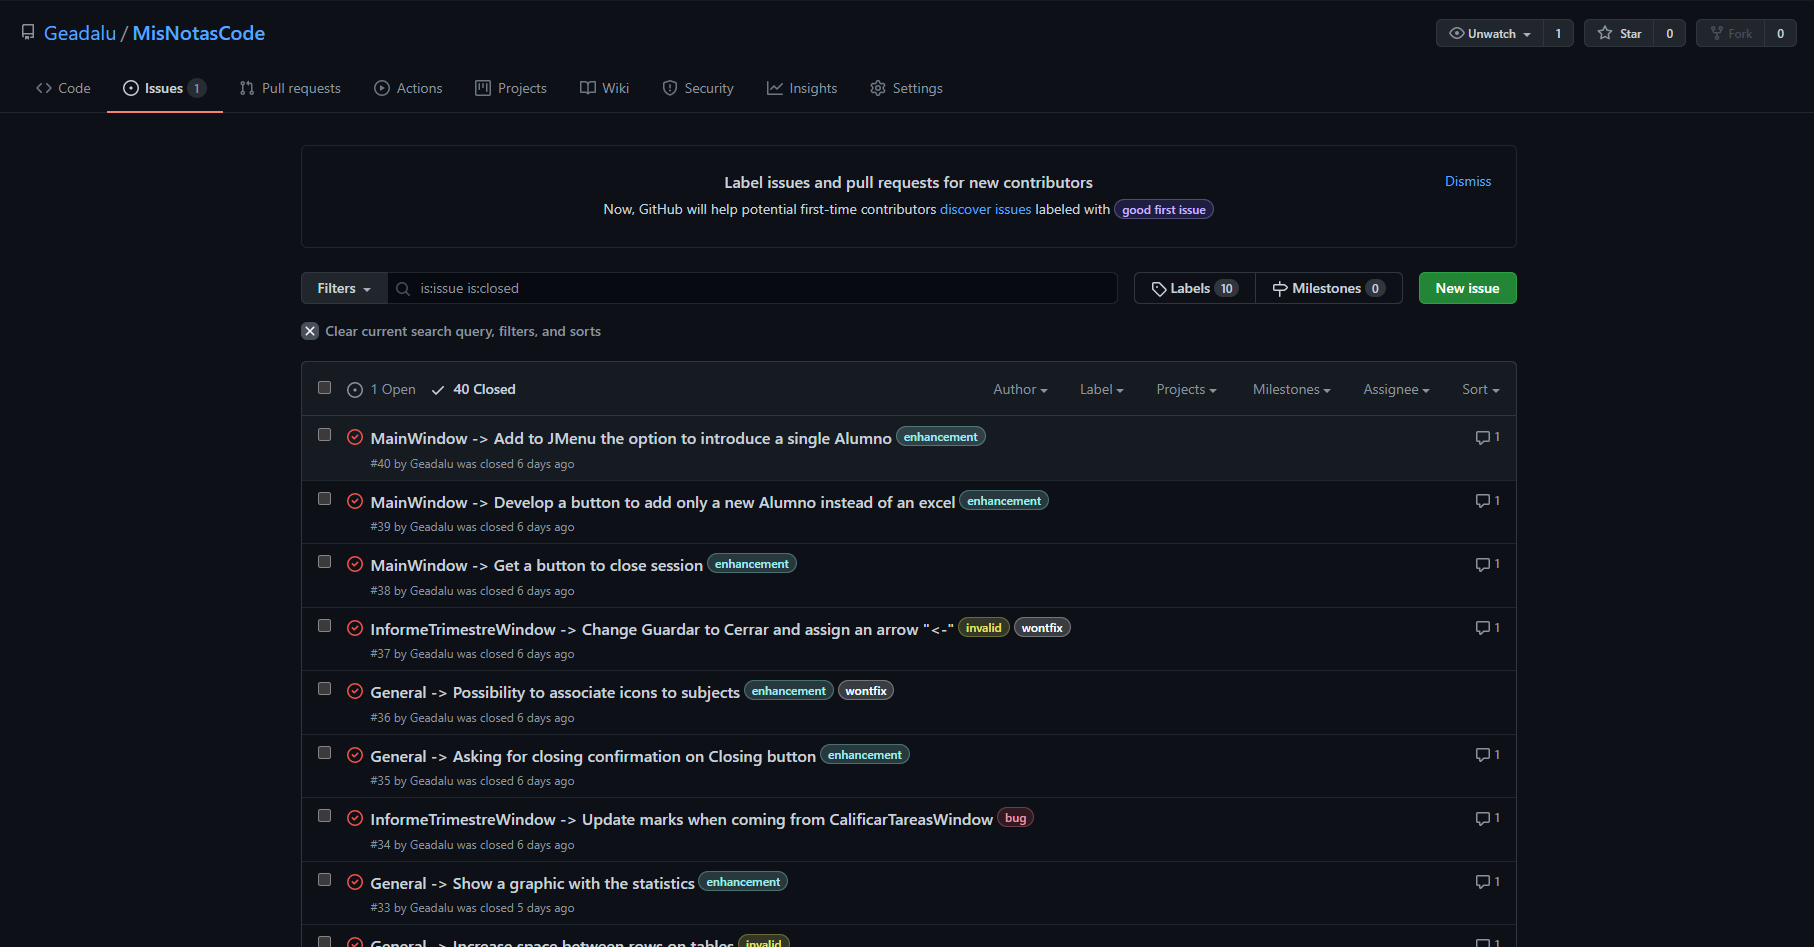
\includegraphics[width=1\linewidth]{figs/github.png}
\caption{Herramienta "Issues" de GitHub. Fuente: \cite{github}}
\label{Fig:issues_github}
\end{figure}

Por último, cabe destacar que también se ha usado la herramienta "Releases", que permite realizar lanzamientos de la aplicación, de manera que los usuarios que visiten el repositorio identificarán rápidamente cuál es la versión que pueden instalarse y ejecutar.


\subsection{Balsamiq Wireframes}
\label{sub:balsamiq}
Para realizar en la fase de Elaboración las maquetas de las interfaces (ver figura \ref{Fig:mockup_mainwindow}), se ha usado la aplicación Balsamiq Wireframes (fuente: \cite{balsamiq}. Esto permite modelar las interfaces de una manera fácil y sencilla. Permite hacer modelos de interfaces para ordenador, tablet y smartphone, y cuenta con una variedad de elementos que se pueden llamar entre sí para realizar una demo.

\subsection{Texmaker y Overleaf}
Se ha optado por los editores de textos Texmaker (ver figura \ref{Fig:texmaker}) y Overleaf para escribir este documento. Texmaker es una apliación de escritorio, que permite escribir y compilar en \LaTeX{}, que es el sistema de composición de textos mediante el cual se ha creado esta memoria.

Texmaker cuenta con el paquete LatexMk, que automatiza la compilación de todas las partes del documento: texto, bibliografía y referencias, y genera el resultado final en un PDF.

Overleaf (fuente: \cite{overleaf}) es, a su vez, un editor de texto para \LaTeX{}, pero web. Se ha decidido usar este cuando se ha tenido que cambiar de sitio de trabajo.

\begin{figure}[h]
\centering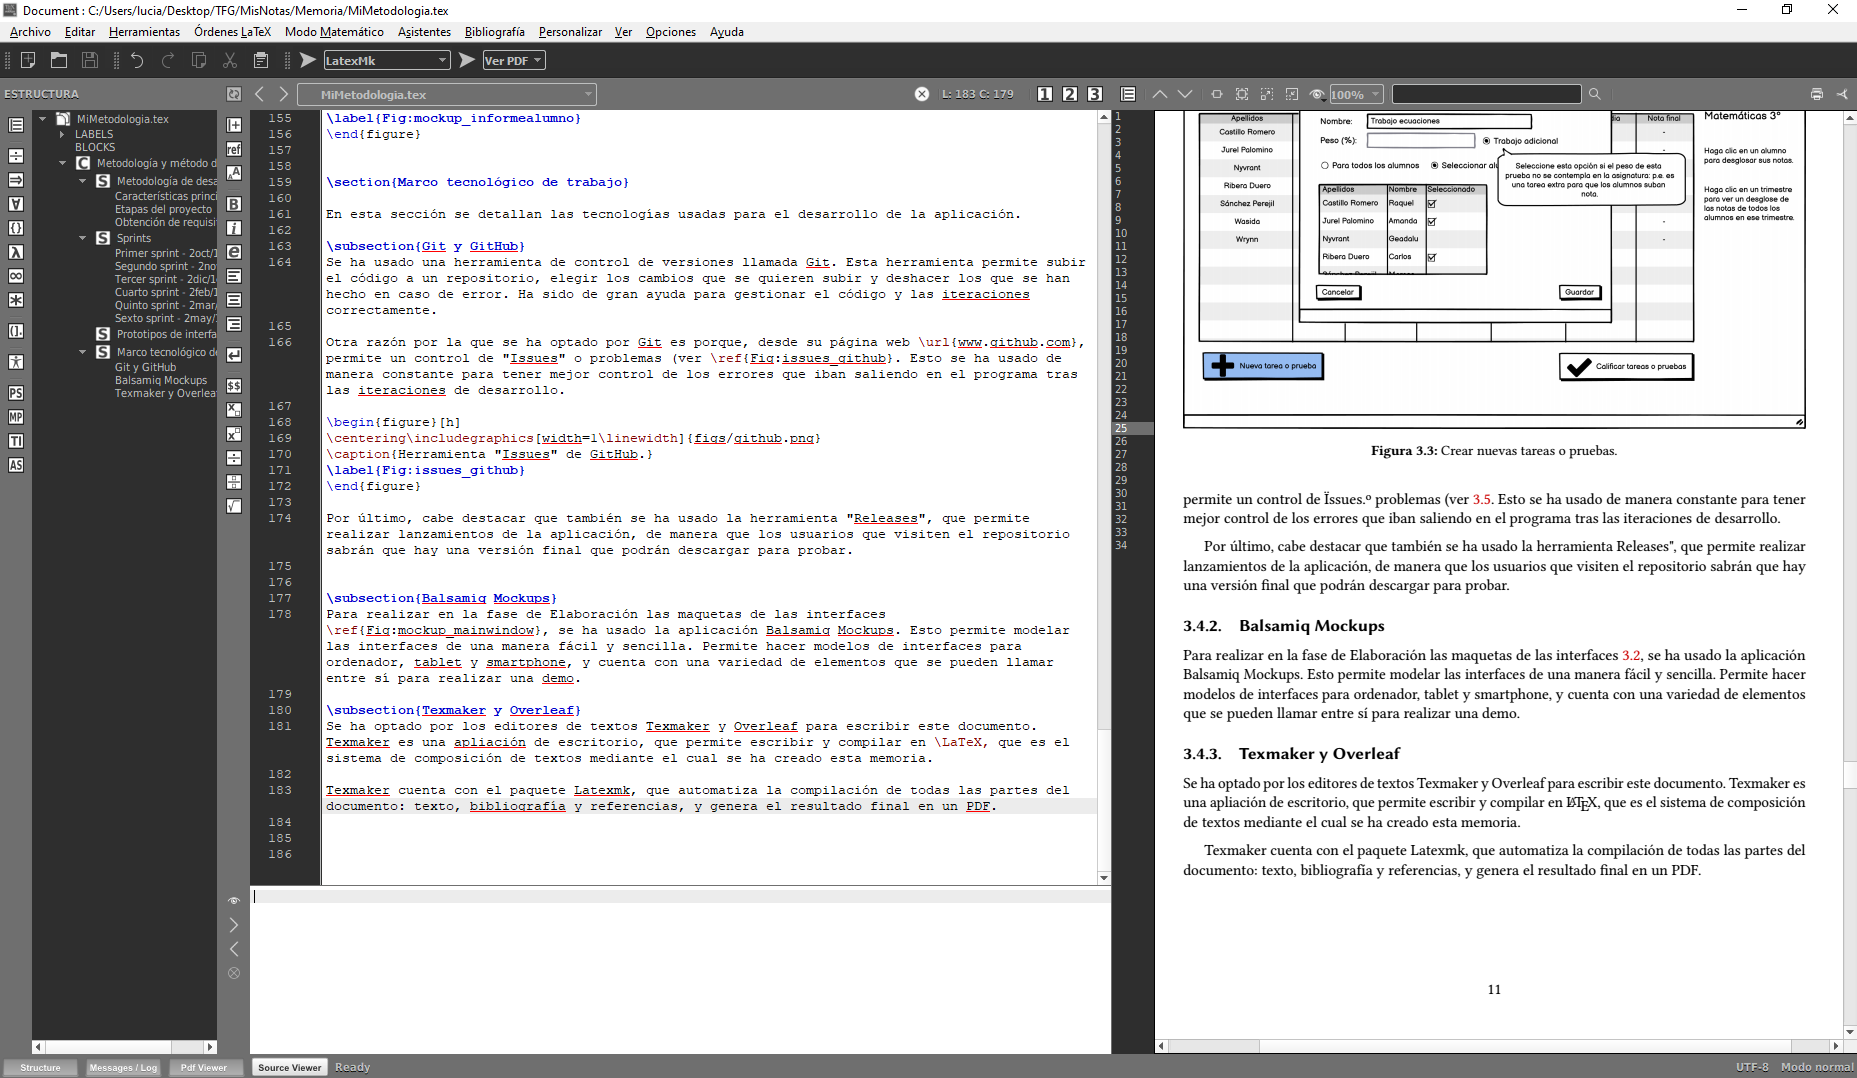
\includegraphics[width=1\linewidth]{figs/Texmaker.png}
\caption{Interfaz del editor de texto Texmaker. Fuente: \cite{texmaker}}
\label{Fig:texmaker}
\end{figure}


\subsection{NetBeans IDE}
Para la escritura de todo el código se ha usado el \gls{ide} gratuito NetBeans (ver figura \ref{Fig:netbeans}).
Este \gls{ide} cuenta con una potente herramienta para realizar las interfaces de los programas en Java, además, es altamente personalizable y tiene conexión con Git al repositorio de GitHub, de tal manera que, en un vistazo, se pueden ver las clases que han cambiado respecto a la versión que hay en GitHub.

\begin{figure}[h]
\centering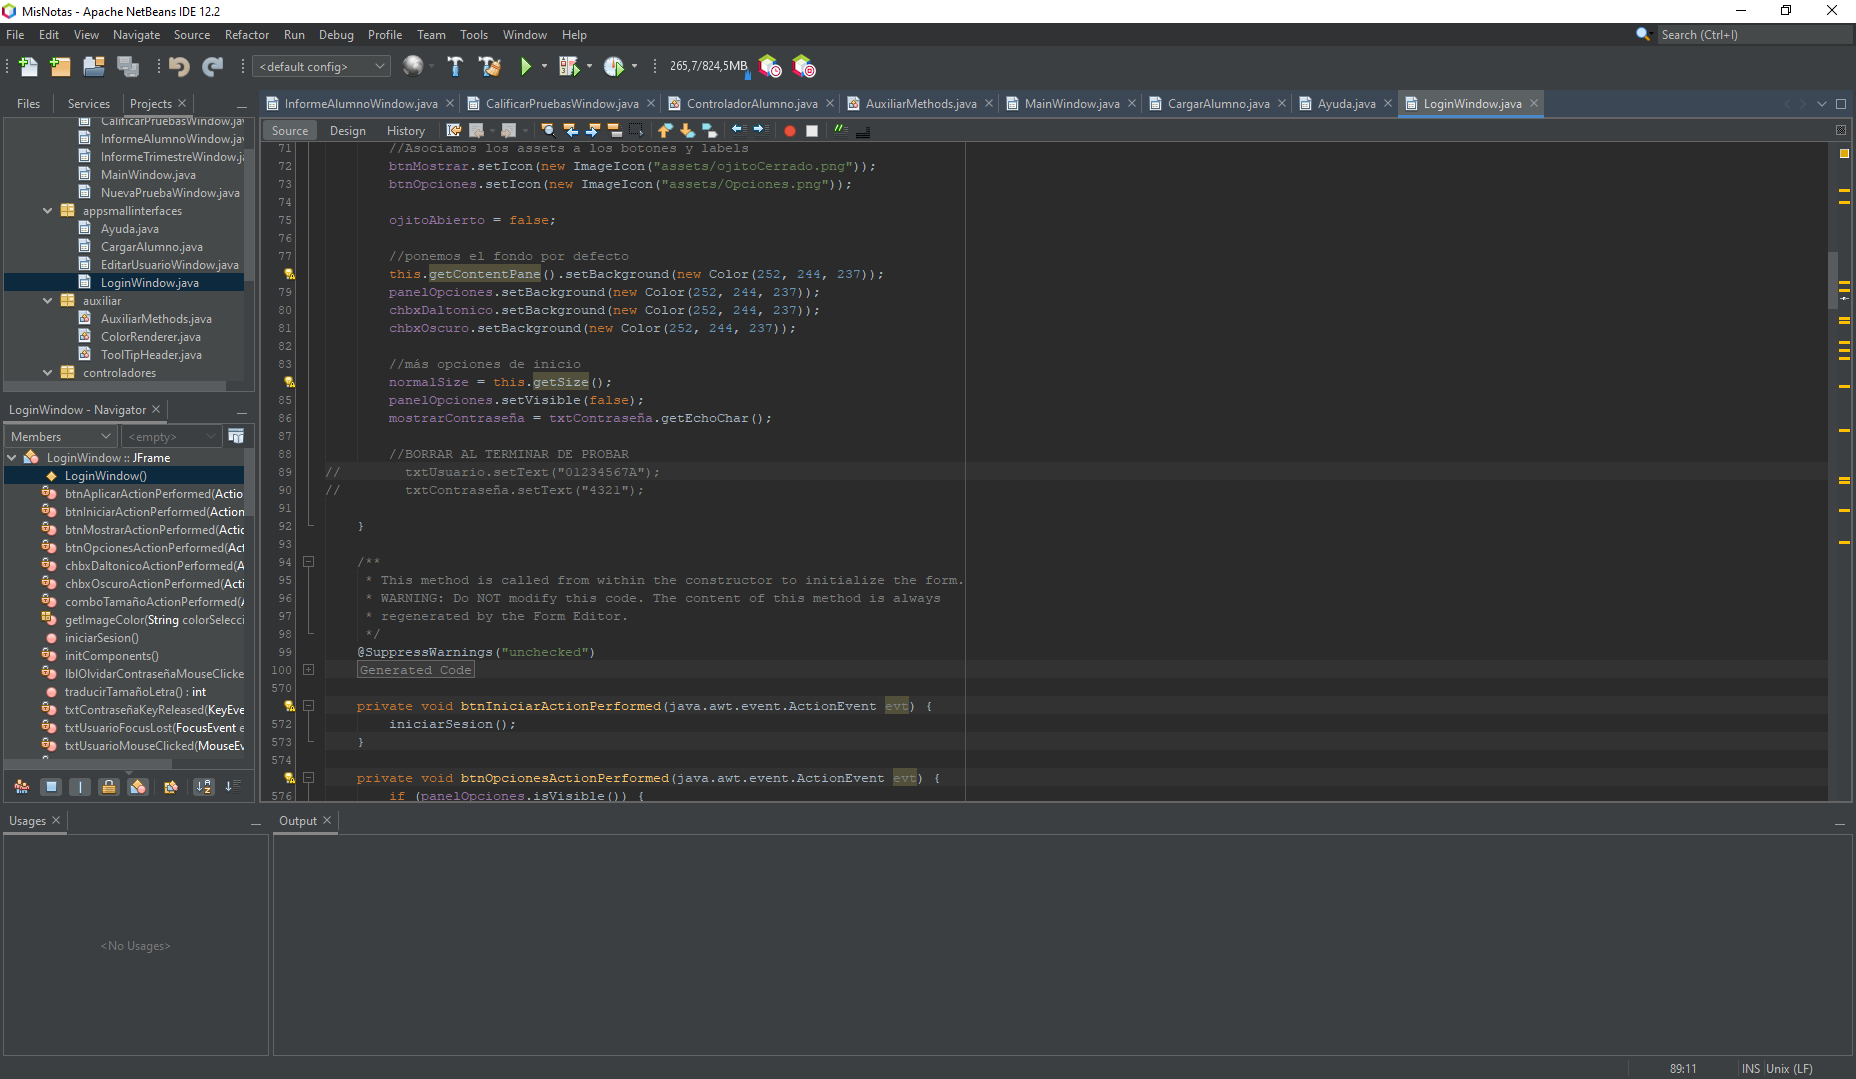
\includegraphics[width=1\linewidth]{figs/netbeans.png}
\caption{Interfaz de NetBeans IDE. Fuente: \cite{netbeans}}
\label{Fig:netbeans}
\end{figure}


\subsection{Procreate}
\label{sub:procreate}
Para el diseño de los iconos e imágenes que se han creado, se ha usado la aplicación de dibujo profesional Procreate (ver figura \ref{Fig:procreate}).

Es una aplicación sencilla e intuitiva que cuenta con varias herramientas para composición de dibujo y pintura.

\begin{figure}[h]
\centering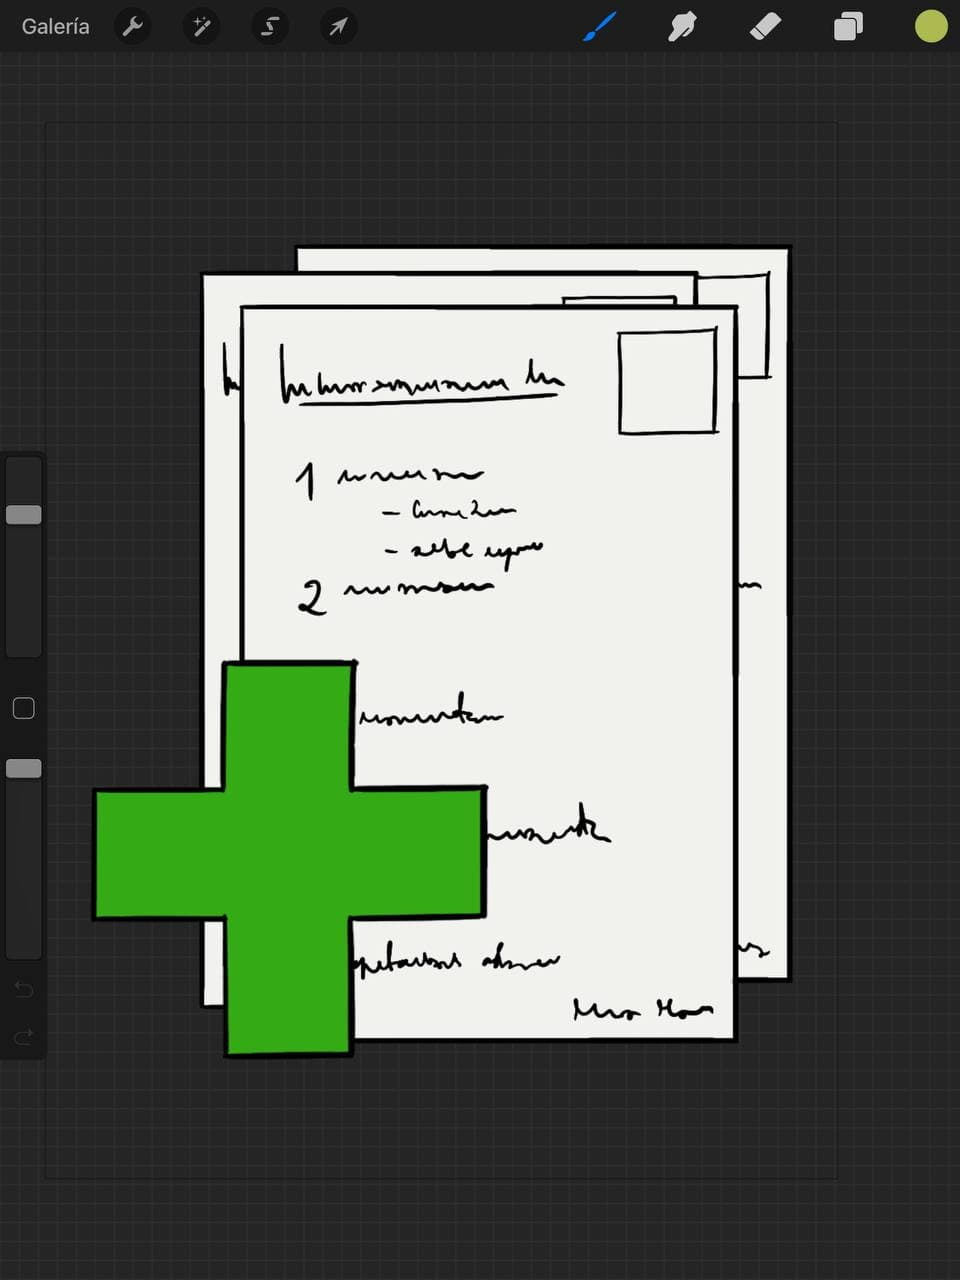
\includegraphics[width=0.5\linewidth]{figs/procreate.jpg}
\caption{Interfaz de dibujo de Procreate. Fuente: \cite{procreate}}
\label{Fig:procreate}
\end{figure}


\subsection{MySQL Workbench}
\label{sub:mysql}
Para la creación y gestión de la base de datos, se ha optado por MySQL Workbench (ver figura \ref{Fig:mysql}). Esta herramienta ha sido verdaderamente útil a la hora de gestionar todos los cambios que se han tenido que ir haciendo a medida que el proyecto iba creciendo, debido a la facilidad de uso y las funcionalidades que posee.

\begin{figure}[h]
\centering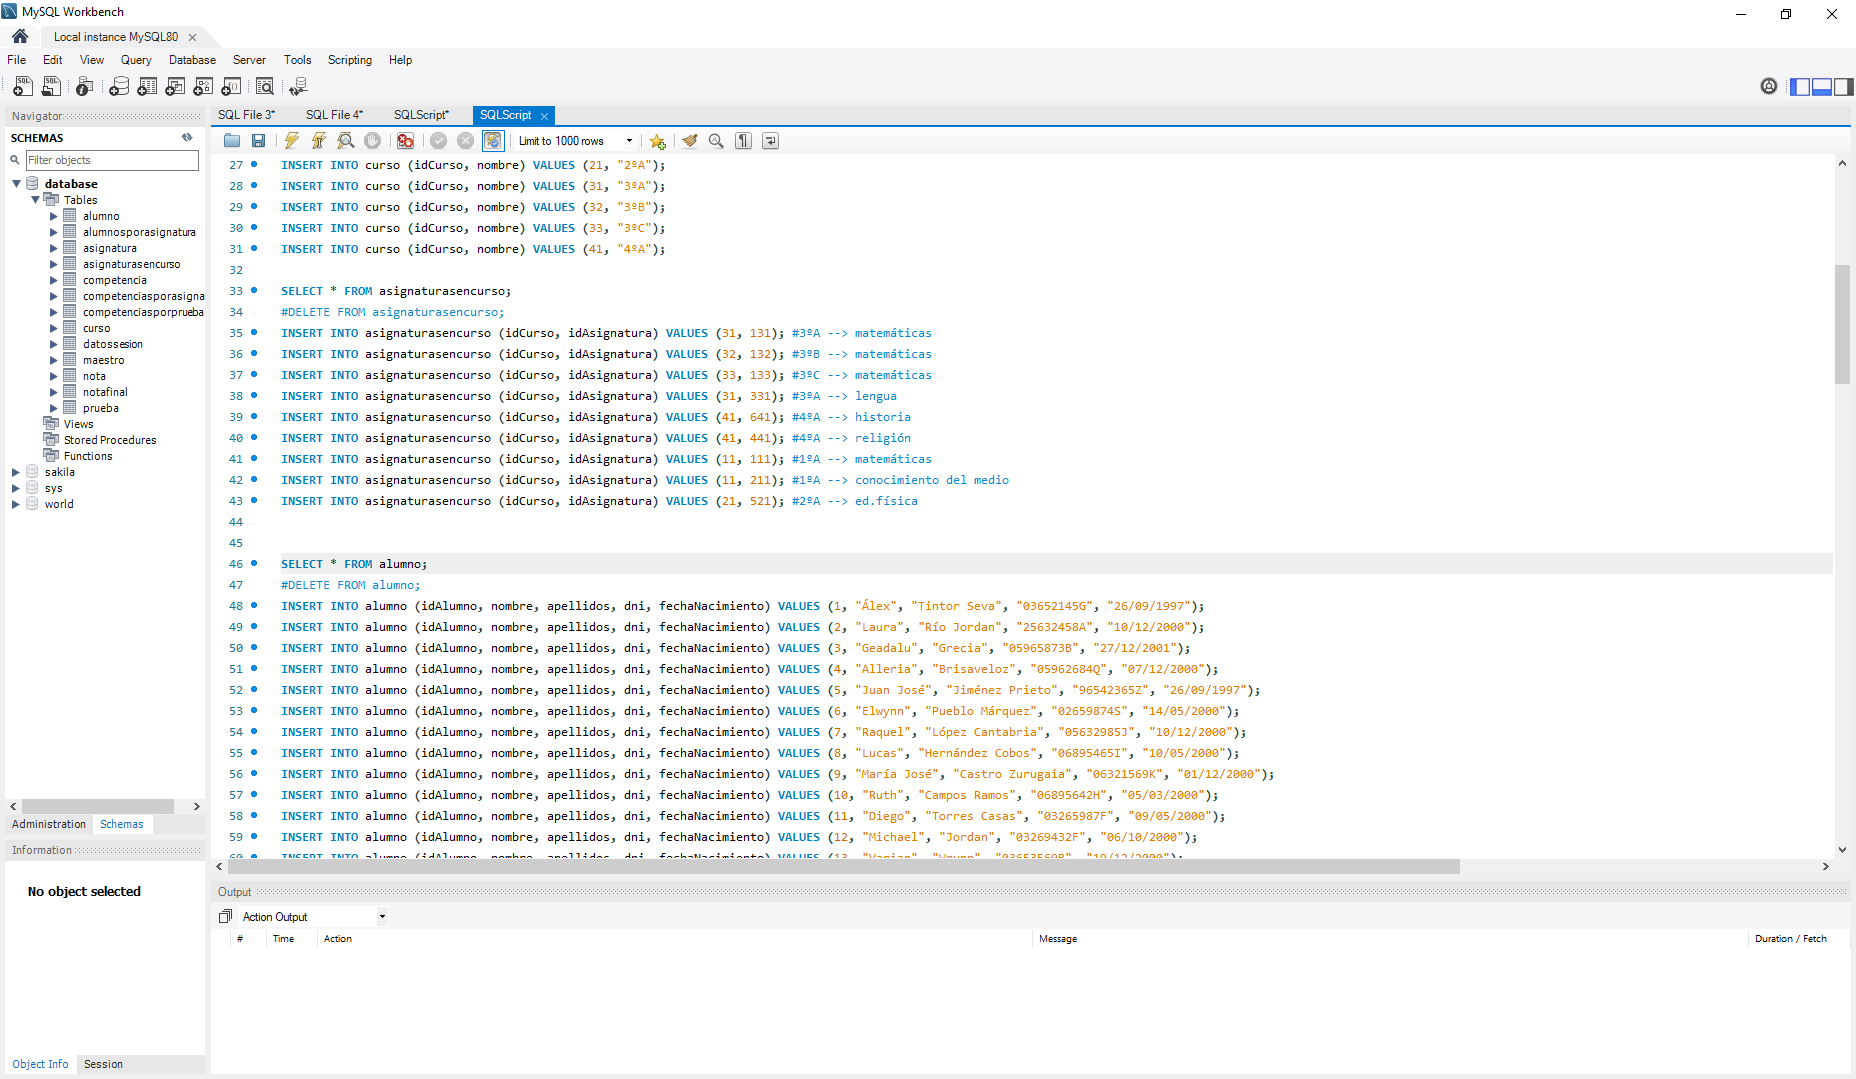
\includegraphics[width=1\linewidth]{figs/mysql.png}
\caption{Interfaz de MySQL Workbench. Fuente: \cite{mysql}}
\label{Fig:mysql}
\end{figure}


\subsection{Otras herramientas}
Cabe mencionar brevemente el uso de otras herramientas que han sido útiles en el desarrollo de este proyecto:
\begin{itemize}
	\item \textbf{tablesgenerator.com:} Como ayuda para la generación de tablas en este documento, se ha usado la herramienta web \url{https://www.tablesgenerator.com/}. Esta página permite crear una tabla de manera visual y generar el código \LaTeX{} correspondiente.
	\item \textbf{paint.net:} es un programa de escritorio para la edición de imágenes de manera básica. Se ha usado para cambiar el tamaño de las imágenes creadas con Procreate o de las sacadas de internet.
	\item \textbf{app.diagrams.net:} potente herramienta web usada para crear todos los diagramas de este documento.
\end{itemize}


\section{Análisis de costes}
\label{sec:analisiscostes}
Como parte de la fase de Inicio de este proyecto, se ha realizado un análisis de costes teniendo en cuenta las tecnologías que se fueran a usar, el tiempo estimado para la finalización del proyecto y otros gastos.

En la mayor parte del desarrollo del proyecto se ha usado software gratuito. Este software incluye: Java, MySQL Workbench, tablesgenerator.com, paint.net, Texmaker y Overleaf, NetBeans IDE, Balsamiq Mockups y Git y Github, mencionados en los apartados anteriores.

Para realizar este análisis de costes, se han tenido en cuenta todas las herramientas y materiales de trabajo, así como el lugar en el que se ha desarrollado y el coste del personal.

En la figura \ref{tab:tablacostes} se muestra una tabla con el software que no ha sido gratuito, así como los diversos costes estimados para el proyecto.

\begin{table}[h]
\caption{Tabla del análisis de costes}
\label{tab:tablacostes}
\begin{tabular}{|l|c|c|c|c|}
\hline
\textbf{Recurso}                                                                                               & \multicolumn{1}{l|}{\textbf{Descripción}}                                                                                                                                         & \multicolumn{1}{l|}{\textbf{\begin{tabular}[c]{@{}l@{}}Precio por \\ unidad\end{tabular}}} & \multicolumn{1}{l|}{\textbf{Unidades}} & \multicolumn{1}{l|}{\textbf{Total}} \\ \hline
\textbf{\begin{tabular}[c]{@{}l@{}}MSI GTX 1060 GAMING X \\ 6GB GDDR5\end{tabular}}                            & \begin{tabular}[c]{@{}c@{}}Tarjeta gráfica instalada\\ en el terminal de trabajo\end{tabular}                                                                                     & 274,98€                                                                                    & 1                                      & 274,98€                             \\ \hline
\textbf{\begin{tabular}[c]{@{}l@{}}Toshiba P300 3.5" 1TB \\ 7200RPM SATA 3\end{tabular}}                       & \begin{tabular}[c]{@{}c@{}}Disco duro instalado\\ en el terminal de trabajo\end{tabular}                                                                                          & 43,99€                                                                                     & 1                                      & 43,99€                              \\ \hline
\textbf{\begin{tabular}[c]{@{}l@{}}Kingston HyperX Fury Black \\ DDR4 2400 PC4-19200 \\ 8GB CL15\end{tabular}} & \begin{tabular}[c]{@{}c@{}}Memoria RAM instalada\\ en el terminal de trabajo\end{tabular}                                                                                         & 70,00€                                                                                     & 2                                      & 140,00€                             \\ \hline
\textbf{Intel Core i5-8400 2.8GHz BOX}                                                                         & \begin{tabular}[c]{@{}c@{}}Procesador instalado\\ en el terminal de trabajo\end{tabular}                                                                                          & 259,90€                                                                                    & 1                                      & 259,90€                             \\ \hline
\textbf{Otros componentes}                                                                                     & \begin{tabular}[c]{@{}c@{}}Otros componentes (cableado, \\ placa base, conector Internet, \\ fuente de alimentación, etc) \\ instalados en el terminal \\ de trabajo\end{tabular} & 230,64€                                                                                    & 1                                      & 230,64€                             \\ \hline
\textbf{Procreate}                                                                                             & \begin{tabular}[c]{@{}c@{}}Aplicación usada en el\\ desarrollo de las figuras\\ de la aplicación\end{tabular}                                                                     & 10,99€                                                                                     & 1                                      & 10,99€                              \\ \hline
\textbf{Alquiler de oficina}                                                                                   & \begin{tabular}[c]{@{}c@{}}Precio mensual del alquiler\\ de una oficina en Madrid\\ para realizar el trabajo\end{tabular}                                                         & 1000,00€                                                                                   & 6                                      & 6.000€                              \\ \hline
\textbf{Coste de personal}                                                                                     & \begin{tabular}[c]{@{}c@{}}Coste horario de la\\ desarrolladora del proyecto\end{tabular}                                                                                         & 9.98€                                                                                      & 350                                    & 3.493€                              \\ \hline
\textbf{Otros costes}                                                                                          & \begin{tabular}[c]{@{}c@{}}Se incluyen: tarifa de luz,\\ material de oficina, etc.\end{tabular}                                                                                   & 150.00€                                                                                    & 1                                      & 150.00€                             \\ \hline
\textbf{COSTE TOTAL}                                                                                           & Suma de la columna Total                                                                                                                                                          & \multicolumn{1}{l|}{}                                                                      & \multicolumn{1}{l|}{}                  & 10.603,50€                          \\ \hline
\end{tabular}
\end{table}


El coste total del proyecto se estima en 10.603,50€(Euros)